\documentclass[english,11pt]{article}
\usepackage{geometry}
\usepackage{setspace}
\geometry{
a4paper,
left=25mm,
right=25mm,
top=25mm,
bottom=25mm,
}
\usepackage[utf8]{inputenc}
\usepackage{babel}
\usepackage{graphicx}
\usepackage[hidelinks]{hyperref}
\usepackage{siunitx}
\usepackage{minted}
\usepackage{eurosym}
\usepackage{amsmath,amssymb}
\usepackage{multirow}
\usepackage{textcomp}
\usepackage{caption}
\usepackage{subcaption}
\usepackage{setspace}

\begin{document}
\onehalfspacing

\setlength{\parindent}{0cm}
\setlength{\parskip}{1ex plus 0.5ex minus 0.2ex}
\newcommand{\hsp}{\hspace{20pt}}
\newcommand{\HRule}{\rule{\linewidth}{0.5mm}}

\begin{titlepage}
  \begin{sffamily}
  \begin{center}

    \textsc{\Large ELEC-H417\\
    Communications networks: protocols and architectures}\\[4.6cm]

    % Title
    \HRule \\[0.4cm]
    { \huge \bfseries Project report \\[0.4cm] }


{\Large Creation of a BitTorrent-like client and tracker\\[3cm]}
  
\begin{center}
\begin{tabular}{l r}
Academic year: & 2016-2017 \\ % Date the experiment was performed
Section: & M-IRELE\\
& \\ \\
Pierre Baudoux & Cédric Hannotier \\
Mathieu Petitjean
\end{tabular}
\end{center}

    \vfill
    % Bottom of the page
    
\includegraphics[width=0.3\textwidth]{img/bruface_logo.png}\\[0.1in]
    \Large{Brussels Faculty of Engineering}\\
    \normalsize
    \textsc{ULB - VUB}\\

    \vspace{0.2cm}

  \end{center}
  \end{sffamily}
\end{titlepage}
\tableofcontents
\newpage

\section{Introduction}
This report presents the implementation of a BitTorrent-like service as a part of the ELEC-H417 course at the Brussels Faculty of Engineering: Communication networks, protocols and architectures.

In this project, two peers (Alice and Bob), a client (Charlie) and a tracker will be implemented. The scheme is represented in Figure \ref{fig:scheme}. 

\begin{figure}[h]
    \centering
    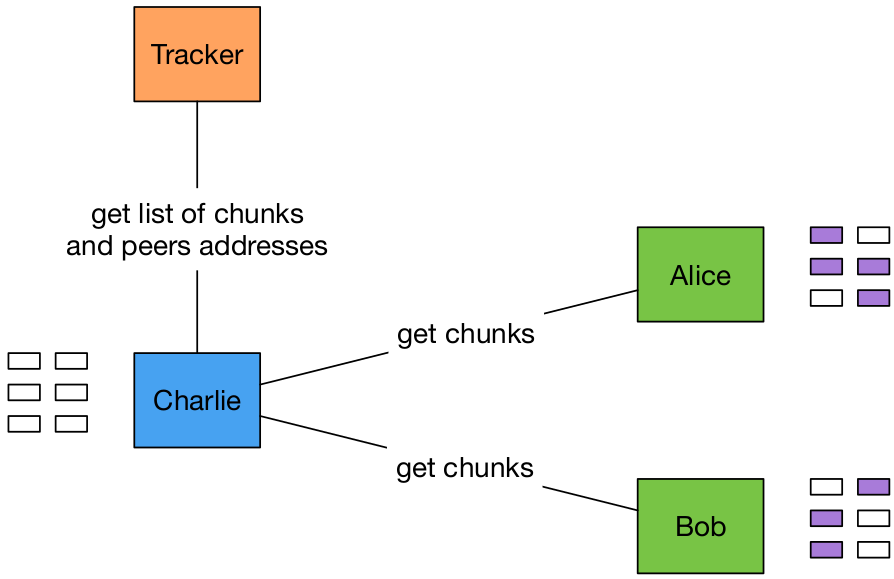
\includegraphics[width = 0.7\textwidth]{img/scheme.png}
    \caption{Scheme of the architecture}
    \label{fig:scheme}
\end{figure}

A file will be split in chunks, which will be distributed between the two peers. The client should be able to connect to the tracker in order to be informed of which peers owns which chunks, and then download the chunks and recover the original file.

The project is divided in three steps, the third one being optional. This report will, for each step, describe the objective of the step, present the description of the proposed solution and its particularities. Moreover, a sequence diagram will be provided.

\newpage

\section{Step 1}
\subsection{Description of the objective}

In the first step, only three entities are created: Alice, Bob and Charlie. The two peers need to read configuration files to know their own IP addresses. The tracker is not implemented yet, the client has to read a configuration file in order to know where the chunks are located.

Knowing the message format used in the project\footnote{\url{https://github.com/jpagex/elec-h-417-project/blob/master/statement.pdf}}
,the peers will analyze the requests they receive from the client and they should be able to either send the chunk that was asked or to return an error message.

\subsection{Proposed solution}

Using object-oriented Python programming, classes \texttt{peers} and \texttt{client} have been created. Alice and Bob are thus \texttt{peers} objects and Charlie is a \texttt{client} object.

All the data transfer between the peers and the clients are handled using TCP to ensure that every requested chunk is correctly transmitted (provided a peer owns it).

\subsubsection{Peers}

The way peers are implemented is quite straightforward. When instantiated, the peer opens a socket and stays idle while waiting for a connection. When a connection is received from the client, a single thread by peer is launched.

This thread will analyze the incoming messages and will send back the appropriate errors when necessary. If the message format and content is correct, the peer will send the requested chunk to the client.

The thread will run and send errors through the socket while there are incoming messages from the client. If the client stops communicating, the peer will assume that all the requests have been sent and it will close the socket and the connection.

\subsubsection{Client}

The client are implemented in order to achieve the maximum file transfer speed, while handling cases where the configuration file declaring which peer owns which chunk is not correct.

Two threads are created so that the chunks are requested and downloaded from Alice and Bob in a parallel way. The library \texttt{Queue} is used, and three queues are created when the client is instantiated. The first and second queues contain the list of chunks that are only owned by one of the two peers. In this way, each thread is sending requests to a different peer and it is only asking for chunks that are not shared. When the queue associated to a thread is empty, it will request chunks that are owned by the two peers, which are listed in the third queue. This implementation allows to ensure that if one the connections is slower that the other, the impact on the file transfer speed will be as little as possible.


\subsection{Sequence diagram}

A simplified version of the sequence diagram of the step 1 code is shown in Figure \ref{fig:step1}. It can be seen that the client uses two threads, each dedicated to the communication with one peer. The interaction with the second peer (Bob) are not shown for sake of clarity, since they are very similar to those concerning the first peer (Alice).

Three specific cases are described : 

\begin{itemize}
	\item Single chunk, no error : the thread gets the chunk to ask in the queue qA, which is filled with chunks only owned by Alice. It sends a request to the corresponding peer. If no error occurs, it tells the queue that the chunk was correctly received.
	
	\item \textit{Multi Chunk}, no error : the thread has finished to ask for chunks listed in qA, and is now getting them for the queue qAB, containing chunks that are supposed to be owned by both peers. The follow-up is the same as in the previous case.
	
	\item \textit{Multi Chunk}, not found error : if the thread is asking for a chunk listed in qAB but Alice responds that she does not actually own it, it is concluded that the other peer (Bob) owns it. It will thus add the given chunk in qB, so that the thread 2 will ask Bob for it.
\end{itemize}

\begin{figure}
	\centering
	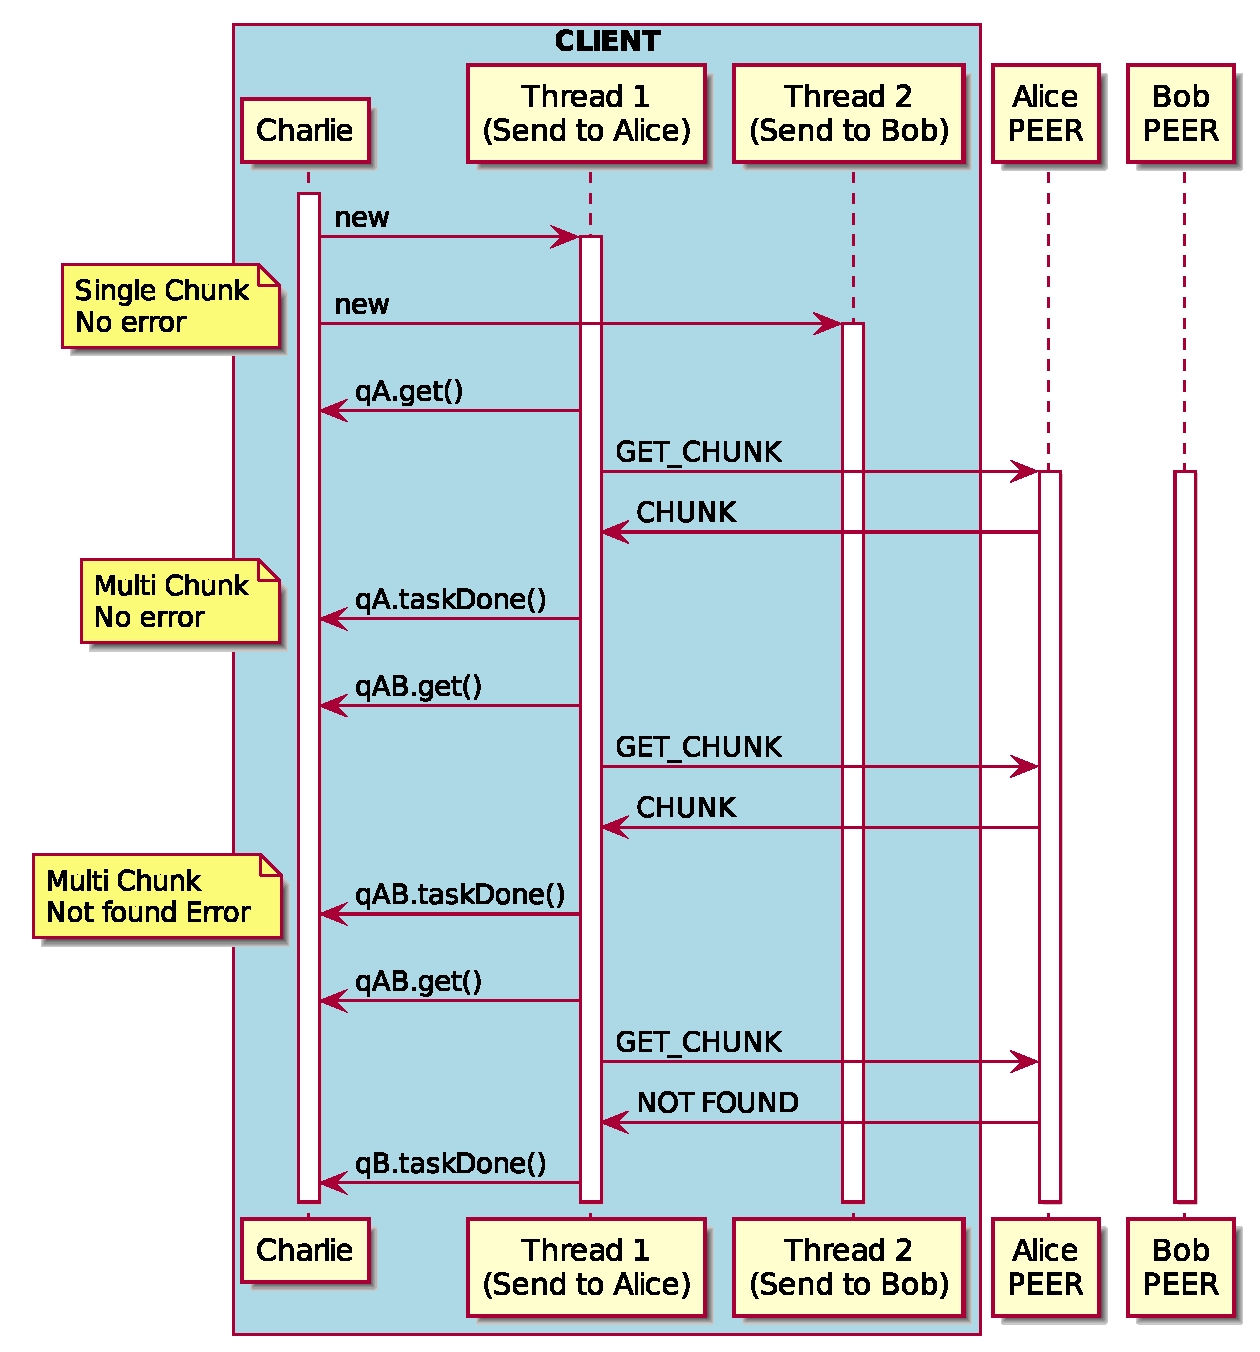
\includegraphics[width=\textwidth]{img/step1.eps}
	\caption{Sequence diagram of step 1}
	\label{fig:step1}
\end{figure}
\newpage

\section{Step 2}
\subsection{Description of the objective}

This step consists of the addition of the tracker. It will provide the client the list of chunks and the peers that own each chunk. The client will thus not have to fetch this information in a configuration file but still needs to know the IP address and port number of the tracker.

\subsection{Proposed solution}

The \texttt{tracker} class now implements the reading of the configuration file as the client did in step 1, in order to know the addresses, ports and chunks of the peers.

When a request is sent by the client to the tracker, all the file information is sent in a message. According to the content of this message, the list of chunks are placed in the adequate queues (only Alice, only Bob or owned by both). The file {\tt file.ini} is created and the follow-up is exactly the same as it was in step 1. The request to the tracker is sent using TCP to ensure that the correct IP and port will be received, as these are essential to establish a connection with the peers.

\subsection{Sequence diagram}

The sequence diagram of the second step is shown in Figure \ref{fig:step2}.

The principle is very similar to the first step once the information of the file is received by the tracker. The connection with the tracker is established similarly to the connection with the peers, and the queues still offer the maximum transfer speed possible.

\begin{figure}
	\centering
	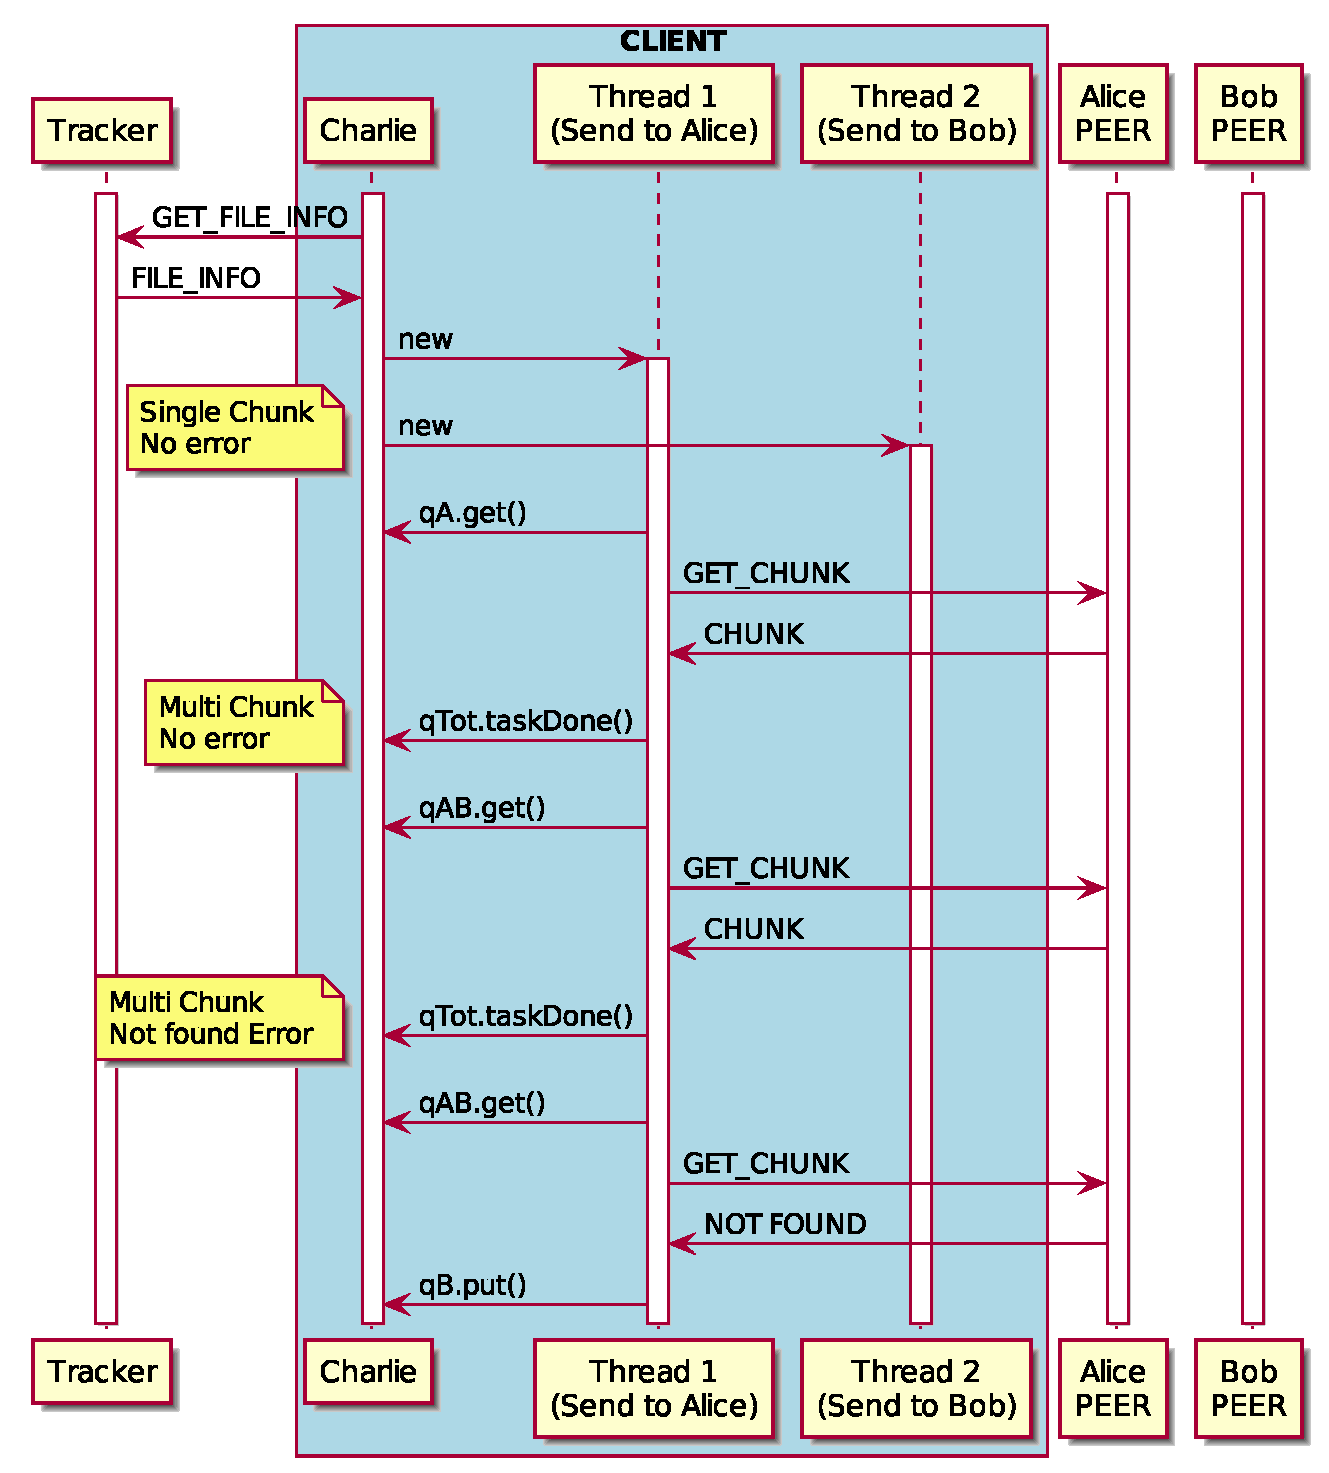
\includegraphics[width=\textwidth]{img/step2.eps}
	\caption{Sequence diagram of step 2}
	\label{fig:step2}
\end{figure}

\subsection{Bonus - contacting the lab tracker}

2 bonus points could be earned by contacting a tracker at the lab and downloading provided in chunks. As the IP address and the port number of this tracker were known, the code of the step 2 was able to contact the tracker, download the chunks and reconstruct the file (5 minutes of the \textit{Start Wars III} movie). It is to be noted that some chunks that were supposed to be owned by both peers were not, but the implementation with the queues allowed to handle it without any problem.



\newpage

\section{Step 3}
\subsection{Description of the objective}

The last step consists of modifying the client and the tracker in such a way that the client will not need a configuration file anymore. The client will instead try to discover the tracker by sending a broadcast message, and the tracker should respond to these discover requests.

\subsection{Proposed solution}

When launched, the tracker is listening to broadcast messages and to TCP requests in separated threads. This broadcast message is sent by the client when wanting to start a file download. The message is sent using UDP because this protocol does not require an established connection between the two agents.

\subsection{Sequence diagram}

The sequence diagram of the third step is shown in Figure \ref{fig:step3}.

The tracker now implements two threads, the first one listening to broadcast message and the second one handling TCP connection with the client as it did in step two.

\begin{figure}
	\centering
	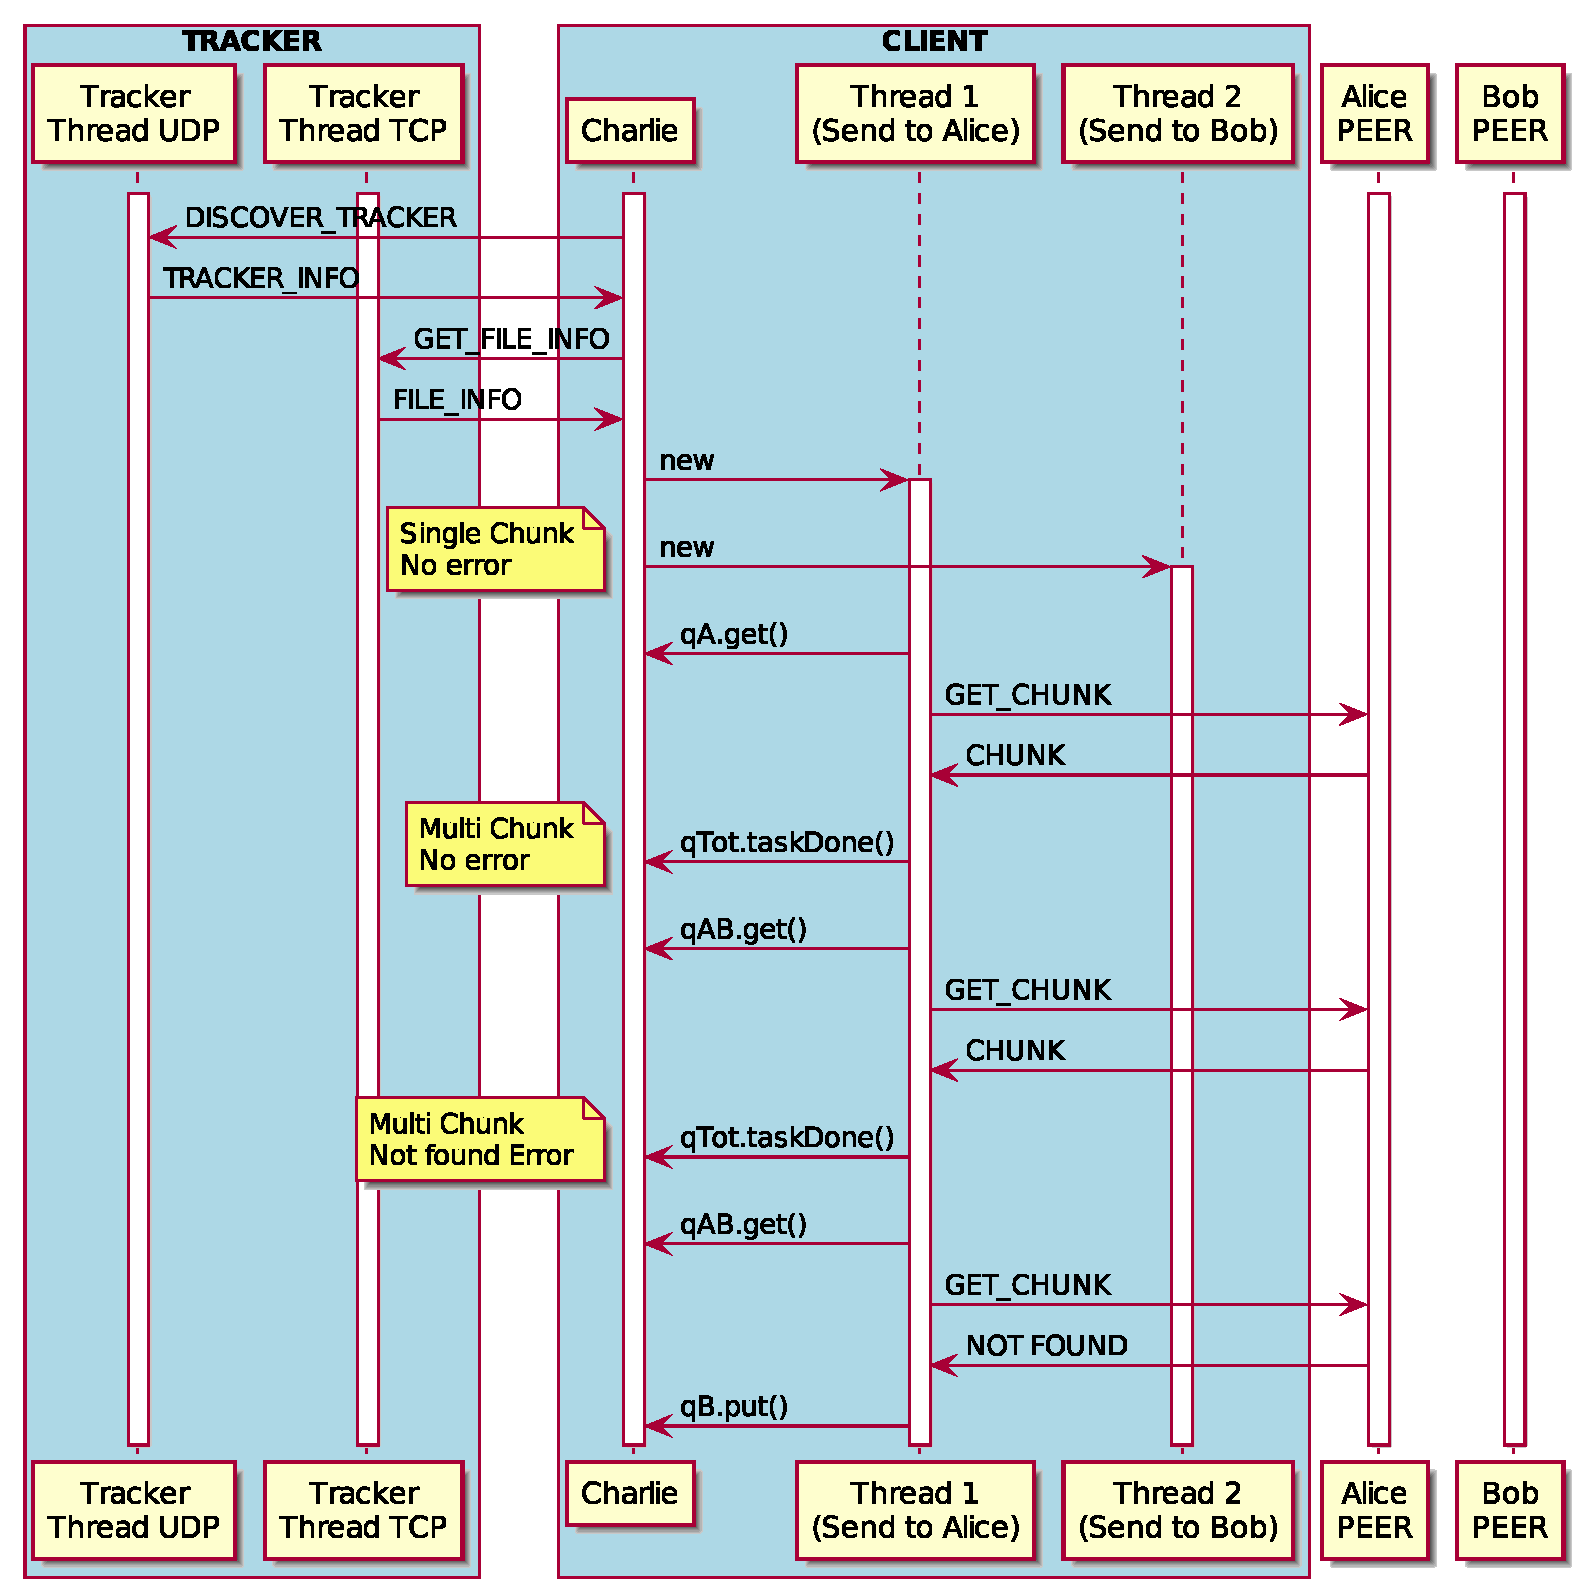
\includegraphics[width=\textwidth]{img/step3.eps}
	\caption{Sequence diagram of step 3}
	\label{fig:step3}
\end{figure}
\newpage
\end{document}
